\documentclass{article}
\usepackage[a4paper, margin=2cm]{geometry}
\usepackage{hyperref}
\usepackage{amsmath, amssymb, commath, physics}
\newcommand{\iu}{\mathbf{i}\mkern1mu}
\newcommand{\ru}{\mathbf{1}\mkern1mu}
\newcommand{\Eu}[1]{\mathbf{e}^{#1}}
\newcommand{\cnorm}[1]{\left|#1\right|}
\newcommand{\conj}[1]{#1^{*}}
\newcommand{\zpolar}[2]{#1\left[\cos\left(#2\right)+\iu\sin\left(#2\right)\right]}

% Colors
\usepackage{xcolor}
\definecolor{xred}{HTML}{BD4242}
\definecolor{xblue}{HTML}{4268BD}
\definecolor{xgreen}{HTML}{52B256}
\definecolor{xpurple}{HTML}{7F52B2}
\definecolor{xorange}{HTML}{FD9337}
\definecolor{xdotted}{HTML}{999999}
\definecolor{xgray}{HTML}{777777}
\definecolor{xcyan}{HTML}{80F5DC}
\definecolor{xpink}{HTML}{F690EA}
\definecolor{xgrayblue}{HTML}{49B095}
\definecolor{xgraycyan}{HTML}{5AA1B9}

% Cancel lines
\usepackage{cancel}
\newcommand\Ccancel[2][red]{
    \let\OldcancelColor\CancelColor
    \renewcommand\CancelColor{\color{#1}}
    \cancel{#2}
    \renewcommand\CancelColor{\OldcancelColor}
}

% Graphics and figures
\usepackage{tikz, pgfplots}
\usetikzlibrary{arrows}
\tikzset{
	vector/.style={-stealth, ultra thick, cap=round},
    coordline/.style={very thick, dotted, black!75},
}
\pgfplotsset{
	compat=1.16,
	%% Styles %%
	xyplane/.style = {
			axis equal,
			axis x line=middle,
			axis y line=middle,
			xlabel=$x$,
			ylabel=$y$,
			every axis x label/.style={at={(ticklabel* cs:1.0)}, anchor=west},
			every axis y label/.style={at={(ticklabel* cs:1.0)}, anchor=south},
			axis line style={stealth-stealth, black, line width=0.5pt},
			% label style={font=\large},
			% tick label style={font=\large},
			samples=250,
			xmin=-5, xmax=5,
			ymin=-5, ymax=5,
			grid=both,
			major grid style={black!5},
			minor grid style={black!2},
			minor tick num = 5,
			xticklabels={,},
			yticklabels={,},
			restrict y to domain=-10:10
		},
    complexplane/.style = {
        xyplane,
        xlabel=$\Re$,
        ylabel=$\Im$,
    },
	xynogrid/.style={
			xyplane,
			major grid style={opacity=0},
			minor grid style={opacity=0},
		},
	xynoaxes/.style={
			xyplane,
			axis line style={draw=none},
			xlabel={}, ylabel={},
			extra x tick labels={,},
			extra y tick labels={,},
			tick style={draw=none},
		},
	xyempty/.style={
			xyplane,
			axis line style={draw=none},
			tick style={draw=none},
			xlabel={},
			ylabel={},
			major grid style={draw=black!0},
		},
}


\setlength{\parindent}{0cm}

\title{Introduction to Complex Numbers and Their Uses}
\author{Peleg Bar Sapir}

\begin{document}
\maketitle

\section{Why Use Complex Numbers?}
Topics:
\begin{enumerate}
	\item From natural numbers to real numbers via extensions (to solve equations).
	\item Square roots for negative real numbers as a justification for imaginary numbers.
	\item The real line as scaling of the unit $\mathbf{1}$ and the imaginary line as scaling of the unit $\iu=\sqrt{-1}$
	\item The real and imaginary sets as orthogonal sets except for $0$.
\end{enumerate}

\section{Algebraic Properties}
\subsection{The complex plane as a vector plane}
\subsection{Addition, multiplication and conjugation of complex numbers}
\textbf{Addition}: let $z=a + b\iu$ and $w=c + d\iu$, then
\begin{equation}
	z+w = a+b\iu + c+d\iu = (a+c) + (b+d)\iu.
	\label{eq:addition_complex}
\end{equation}

\textbf{Multiplication}: let $z=a + b\iu$ and $w=c + d\iu$, then
\begin{equation}
	\begin{aligned}
		z \cdot w & = (a+b\iu)(c+d\iu)                \\
		          & = ac + ad\iu + b\iu c + b\iu d\iu \\
		          & = ac + (ad+bc)\iu + bd\iu^{2}     \\
		          & = ac + (ad+bc)\iu - bd            \\
		          & = ac-bd + (ad+bc)\iu.
	\end{aligned}
	\label{eq:multiplication_complex}
\end{equation}

\textbf{Dividing by $\iu$}: to find what is $\frac{1}{\iu}$ we can just multiply the fraction by $\frac{\iu}{\iu}$ (since $\frac{x}{x}=1$ for any $x\neq0$):
\begin{equation}
	\frac{1}{\iu} = \frac{1}{\iu}\cdot\frac{\iu}{\iu} = \frac{\iu}{\iu\cdot\iu} = \frac{\iu}{\iu^{2}} = \frac{\iu}{-1} = -\iu.
	\label{eq:1_over_i}
\end{equation}

\textbf{Norm}: we can define the norm of a complex number in a similar way to that of vectors in $\mathbf{R}^{2}$, i.e. for $z=a+b\iu$
\begin{equation}
	\cnorm{z}^{2} = a^{2}+b^{2}.
	\label{eq:complex_norm}
\end{equation}

\textbf{Conjugate}: we define a new property of a complex number $z=a+b\iu$ called its \textbf{conjugate}, $\conj{z}$:
\begin{equation}
	\conj{z} = a - b\iu.
	\label{eq:complex_conjugate}
\end{equation}
(see \autoref{fig:conjugate})

We can then define the square norm of a complex number $z$ to be
\begin{equation}
	\cnorm{z}^{2} = z\conj{z},
	\label{eq:complex_norm_via_conj}
\end{equation}
since for $z=a+b\iu$ we get
\begin{equation}
	z\conj{z} = (a+b\iu)(a-b\iu) = a^{2} - \Ccancel{ab\iu + b\iu a} - b^{2}{\iu^{2}} = a^{2}+b^{2} = \cnorm{z}^{2}.
	\label{eq:complex_norm_via_conj_explaination}
\end{equation}

\begin{figure}
	\begin{center}
		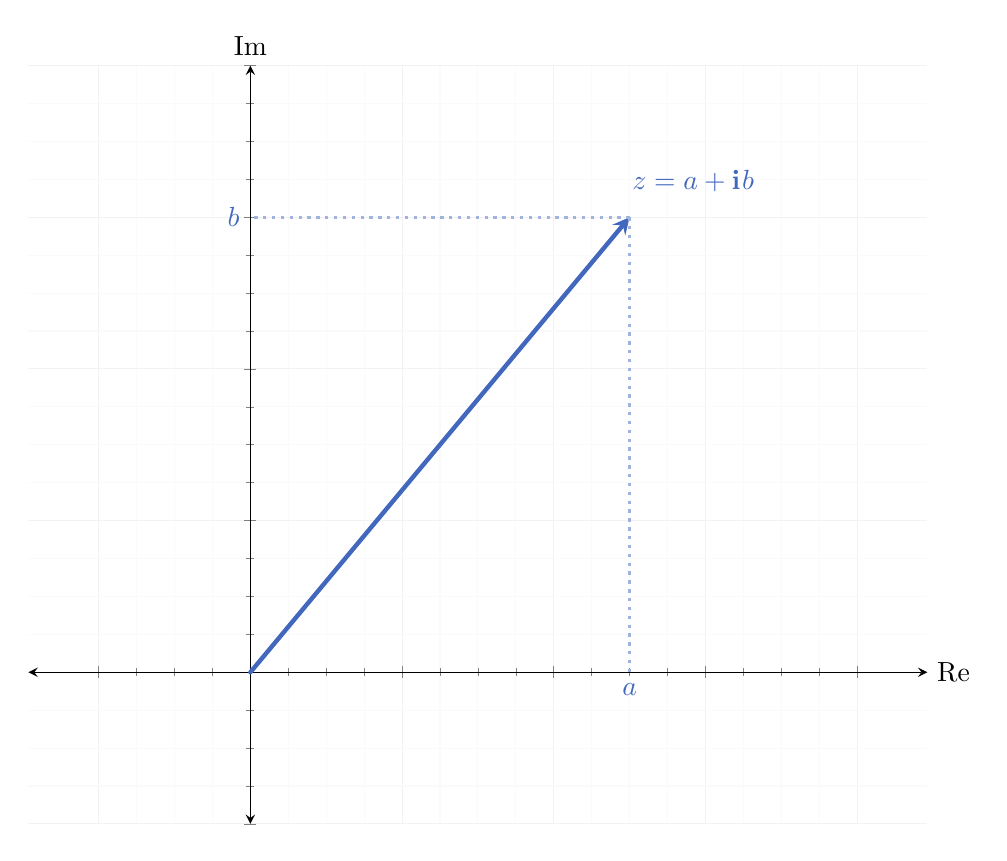
\begin{tikzpicture}[scale=1]
			\def\zcol{xblue}
			\begin{axis}[
					width=13cm,
					complexplane,
					xmin=-1, xmax=4,
					ymin=-1, ymax=4,
					xtick={-1,...,4},
					ytick={-1,...,4},
					minor tick num=3,
				]
				\pgfmathsetmacro{\a}{2.5}
				\pgfmathsetmacro{\b}{3.0}
				\draw[vector, \zcol] (0,0) -- (\a,\b) node [anchor=west, pos=1.05, xshift=-10pt, yshift=5pt] (z) {$z=a+\iu b$};
				\draw[coordline, \zcol!50] (\a,\b) -- (\a,0) node[below, \zcol] {$a$};
				\draw[coordline, \zcol!50] (\a,\b) -- (0,\b) node[left, \zcol] {$b$};
			\end{axis}
		\end{tikzpicture}
	\end{center}
	\caption{This is a test figure.}
	\label{fig:testfig}
\end{figure}

\begin{figure}
	\begin{center}
		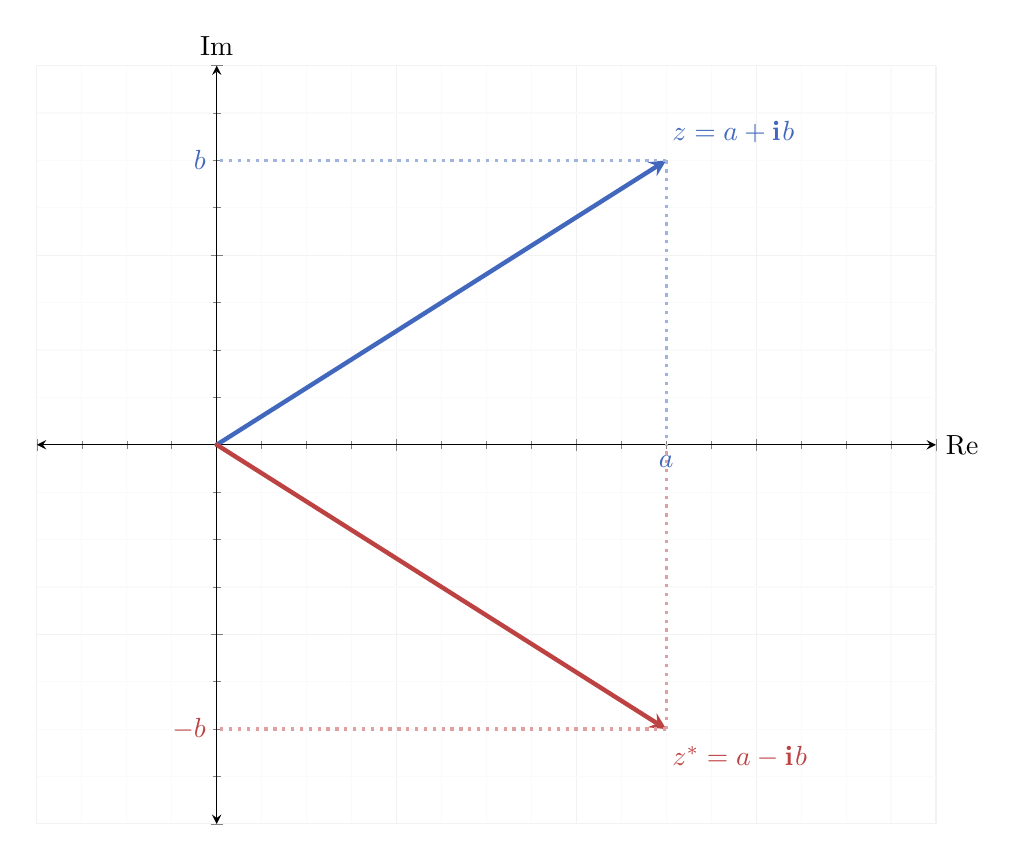
\begin{tikzpicture}[scale=1]
			\def\zcol{xblue}
			\def\zconjcol{xred}
			\begin{axis}[
					width=13cm,
					complexplane,
					axis equal=false,
					xmin=-1, xmax=4,
					ymin=-2, ymax=2,
					xtick={-1,...,4},
					ytick={-2,...,2},
					minor tick num=3,
				]
				\pgfmathsetmacro{\a}{2.5}
				\pgfmathsetmacro{\b}{1.5}
				\draw[vector, \zcol] (0,0) -- (\a,\b) node [anchor=west, pos=1.05, xshift=-10pt, yshift=5pt] (z) {$z=a+\iu b$};
				\draw[vector, \zconjcol] (0,0) -- (\a,-\b) node [anchor=west, pos=1.05, xshift=-10pt, yshift=-5pt] (zconj) {$\conj{z}=a-\iu b$};
				\draw[coordline, \zcol!50] (\a,\b) -- (\a,0) node[below, \zcol] {$a$};
				\draw[coordline, \zcol!50] (\a,\b) -- (0,\b) node[left, \zcol] {$b$};
				\draw[coordline, \zconjcol!50] (\a,-\b) -- (\a,0);
				\draw[coordline, \zconjcol!50] (\a,-\b) -- (0,-\b) node[left, \zconjcol] {$-b$};
			\end{axis}
		\end{tikzpicture}
	\end{center}
	\caption{Complex conjugate of $z=a+b\iu,\ \conj{z}=a-b\iu$.}
	\label{fig:conjugate}
\end{figure}

\section{Polar (Geomteric) Representation}
% \begin{enumerate}
% 	\item Norm and angle as vector polar coordinates.
% 	\item Transforming $z=a+\iu b$ into polar coordinates and back.
% 	\item Multiplication of complex numbers in polar form: scaling and rotation (real and imaginary parts, respectively).
% 	\item Using the polar form to find complex roots.
% \end{enumerate}
\subsection{Norm and angle}
Just like with vectors in $\mathbb{R}^{2}$, we can use the polar coordinates system to describe a complex number $z=a+b\iu$: we take the norm of the number $\cnorm{z}$ as the first coordinate, and its angle with the real axis as the second coordinate (see REF).

The correspondence between the Cartesian coordinates and polar coordinates are as follows:
\begin{equation}
	\begin{aligned}
		\Re{z} & = r\cos\left(\varphi\right), \\
		\Im{z} & = r\sin\left(\varphi\right). \\
	\end{aligned}
	\label{polar_to_cartesian_trans}
\end{equation}
Thus, instead of writing $z=a+b\iu$, we can write
\begin{equation}
	z = r\cos(\varphi) + r\sin(\varphi)\iu = \zpolar{r}{\varphi}.
	\label{eq:}
\end{equation}

This gives as the following Transformation rules between the coordinate systems:
\begin{equation}
	\begin{aligned}
		r = \cnorm{z} = \sqrt{a^{2}+b^{2}}, \\
		\varphi = \arctan\left(\frac{\Im{z}}{\Re{z}}\right).
	\end{aligned}
	\label{eq:cartesian_to_polar_trans}
\end{equation}

Multiplication of complex numbers becomes very simple in polar form: let $z_{1}=\zpolar{r_{1}}{\varphi_{1}}$ and $z_{2}=\zpolar{r_{2}}{\varphi_{2}}$. We then get
\begin{equation}
	\begin{aligned}
		z_{1}\cdot z_{2} & = \zpolar{r_{1}}{\varphi_{1}}\cdot\zpolar{r_{2}}{\varphi_{2}}                                                                                                                                                  \\
		                 & = r_{1}r_{2}\left[\cos\left(\varphi_{1}\right)\cos\left(\varphi_{2}\right) + \iu\cos(\varphi_{1})\sin(\varphi_{2}) + \iu\sin(\varphi_{1})\cos(\varphi_{2}) + \iu^{2}\sin(\varphi_{1})\sin(\varphi_{2}) \right] \\
		                 & = r_{1}r_{2}\left[\cos(\varphi_{1})\cos(\varphi_{2})-\sin(\varphi_{1})\sin(\varphi_{2}) + \iu\left[\cos(\varphi_{1})\sin(\varphi_{2})+\sin(\varphi_{1})\cos(\varphi_{2})\right]\right].
	\end{aligned}
	\label{eq:complex_product_polar_form_part_1}
\end{equation}
Recall the following two trigonometric identites:
\begin{equation}
	\begin{aligned}
		\cos(a)\cos(b)-\sin(a)\sin(b) & = \cos(a+b), \\
		\cos(a)\sin(b)+\sin(a)\cos(b) & = \sin(a+b).
	\end{aligned}
	\label{eq:trig_identites}
\end{equation}

Using these two identites, \autoref{eq:complex_product_polar_form_part_1} becomes very simple:
\begin{equation}
	z_{1}z_{2} = r_{1}r_{2}\zpolar{}{\varphi_{1}+\varphi_{2}}.
	\label{eq:complex_product_polar_form_part_2}
\end{equation}

We can interpret the product of two complex numbers using \autoref{eq:complex_product_polar_form_part_2} as \textbf{scaling} $z_{1}$ by the norm of $z_{2}$, and \textbf{rotating} it by the angle of $z_{2}$ (or vice-versa, since the product is commutative).

(FIGURE?)

\section{Exponential Representation}
\subsection{Euler's Forumla}
Exponentiating $\iu$ with non-negative integers yields the following pattern:
\begin{align*}
	\iu^0 & = 1    \\
	\iu^1 & = \iu  \\
	\iu^2 & = -1   \\
	\iu^3 & = -\iu \\
	\iu^4 & = 1    \\
	\iu^5 & = \iu  \\
	\iu^6 & = -1   \\
	\iu^7 & = -\iu \\
	      & \vdots
\end{align*}
i.e. we get the infinitely repeating sequence ${1, \iu, -1, -\iu}$.

Now, the Taylor series of sine and cosine around $x_{0}=0$:
\begin{alignat}{2}
	\cos(x) & = \sum\limits_{k=0}^{\infty} \frac{(-1)^{n}}{(2n)!}x^{2n}     & = 1 - \frac{x^2}{2!} + \frac{x^4}{4!} - \frac{x^6}{6!} + \dots \\
	\sin(x) & = \sum\limits_{k=0}^{\infty} \frac{(-1)^{n}}{(2n+1)!}x^{2n+1} & = x-\frac{x^3}{3!}+\frac{x^5}{5!} - \frac{x^7}{7!} + \dots
	\label{eq:cosine_and_sine_taylor}
\end{alignat}

And of the exponential function $f(x)=\Eu{x}$ is
\begin{equation}
	\Eu{x} = \sum\limits_{k=0}^{\infty} \frac{x^{k}}{k!} = 1 + x + \frac{x^2}{2} + \frac{x^3}{3!} + \frac{x^4}{4!} + \dots
	\label{eq:exp_taylor}
\end{equation}

Therefore, a generic complex number has the polar form
\begin{equation}
	\begin{aligned}
		z & = R \left( \cos(\theta) + \iu\sin(\theta) \right)                                                                                                                                       \\
		  & = R \left(1 - \frac{x^2}{2!} + \frac{x^4}{4!} - \frac{x^6}{6!} + \dots + \iu\left[x-\frac{x^3}{3!}+\frac{x^5}{5!} - \frac{x^7}{7!} + \dots\right] \right)                               \\
		  & = R\left(1 + \iu x - \frac{x^2}{2!} - \frac{x^3}{3!} + \frac{x^4}{4!} + \iu\frac{x^5}{5!} - \frac{x^6}{6!} - \frac{x^7}{7!} + \dots \right)                                             \\
		  & = R\left(\iu^0 + \iu^1 x + \iu^2 \frac{x^2}{2!} + \iu^3 \frac{x^3}{3!} + \iu^4 \frac{x^4}{4!} + \iu^5 \frac{x^5}{5!} + \iu^6 \frac{x^6}{6!} + \iu^7 \frac{x^7}{7!} + \dots \right)      \\
		  & = R\left((\iu x)^0 + (\iu x)^1 + \frac{(\iu x)^2}{2!} + \frac{(\iu x)^3}{3!} + \frac{(\iu x)^4}{4!} + \frac{(\iu x)^5}{5!} + \frac{(\iu x)^6}{6!} + \frac{(\iu x)^7}{7!} + \dots\right) \\
		  & = R\Eu{\iu x}.
	\end{aligned}
	\label{eq:}
\end{equation}

% \begin{enumerate}
% 	\item The Taylor series of $\cos(\theta), \sin(\theta)$ and $\exp(\theta)$, and how $\exp(\iu\theta)=\cos(\theta)+\iu\sin(\theta)$. How $\exp(\iu\pi)+1=0$.
% 	\item The complex exponential function $f(t)=\exp(\iu t)$ as the "better form" of $\sin(t)$ and $\cos(t)$ (with matplotlib animations).
% 	\item The behaviour of the general $f(t) = \exp(z)$ function (where $z\in\mathbb{C}$).
% \end{enumerate}

\section{Introduction to Fourier Transforms}
\begin{enumerate}
	\item How we can compose different sines and cosines to get complicated functions (Fourier series).
	\item From Fourier series to Fourier Transforms (FTs), and using FTs to filter/compress data (just examples).
	\item The complex polar form of Fourier series (only imaginary terms).
	\item How we can use Fourier series to draw closed shapes in 2D (it's really cool!).
\end{enumerate}

\section{Complex Functions?}
\section{Higher-dimension Forms: Quaternions, Octanions, Clifford Algebras?}

\end{document}
